\newpage
\section{Classification Rules}
%\begin{figure}[H]
%  \centering
%  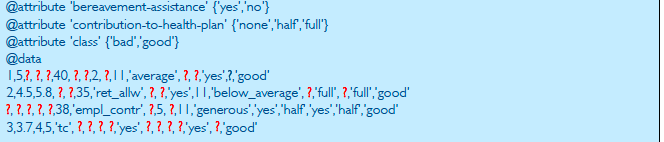
\includegraphics[width=.5\linewidth]{arffmissing}
%\end{figure}
Given a dataset
\begin{figure}[H]
  \centering
  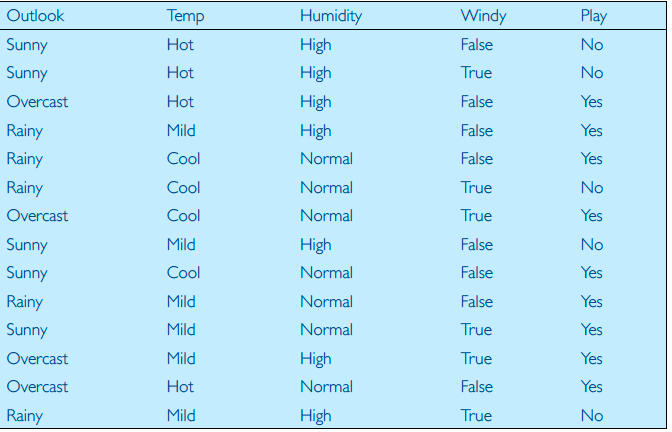
\includegraphics[width=.5\linewidth]{weatherdata}
\end{figure}
A set of \textbf{rules} can be used to classify data:
\begin{itemize}
\item IF (humidity = high) AND (outlook = sunny) THEN play=no (3.0/0.0)
\item IF (outlook = rainy) AND (windy = TRUE) THEN play = no (2.0/0.0)
\item OTHERWISE play = yes (9.0/0.0)
\end{itemize}
A classification rule are \textbf{IF-THEN rules} where the IF part states conditions (\textbf{propositional with comparison and FOL Horn clauses}) over data and the THEN part includes a class label. \\
A classification rule is characterized by :
\begin{itemize}
\item \textbf{ncovers} = number of examples covered by the rule
\item \textbf{ncorrect} = number of examples correctly classified by the rule
\item \textbf{coverage(R)} = $\frac{\text{ncovers}}{\text{size of training data set}}$
\item \textbf{accuracy(R)} = $\frac{\text{ncovers}}{\text{ncorrect}}$
\end{itemize}
If more than 1 rule is triggered a \textbf{conflict} can happen and must be solved:
\begin{itemize}
\item \textbf{Size ordering} = assign highest priority to the triggering rule that has the \textbf{toughest} requirements ( = with the most attribute test)
\item \textbf{Class-based ordering} = decreasing order of \textbf{prevalence} or \textbf{missclassification cost} per class
\item \textbf{Rule-based ordering} = rules are organized into a long priority list according to some measure of rule quality
\end{itemize}
Rule learning can be done in two ways:
\begin{itemize}
\item \textbf{Direct Method} = directly learn the rules from the training data
\item \textbf{Indirect Methods} = learn decision trees or NN and from there convert/extract rules
\end{itemize}

\subsection{Direct Method}
\subsubsection{IR Classifier}
IR Classifier learns a simple rule involving \textbf{one attribute} (assumes \textbf{nominal} attributes) in a similar way to a decision stump. The rule tests \textbf{all values} of one particular attribute.
\begin{enumerate}
\item One branch for each value
\item Each branch assigns most frequent class
\item Performance measured using \textbf{error rate}	computed as the proportion of instances that don't belong to the majority class of their corresponding branch. Missing value = separate value.
\item Choose attribute with lowest error rate	
\end{enumerate}
\textbf{Numerical attributes} can be used but must be \textbf{discretized} : decreases complexity but at the cost of losing some information. IR applies \textbf{supervised discretization} :
\begin{itemize}
\item Sort instances according to \textbf{attribute's value}
\item Place \textbf{breakpoints} where class changes (majority class)
\end{itemize}
This procedure is \textbf{very sensitive to noise} and can lead to \textbf{overfitting} . To avoid this a \textbf{minimum number} of instances can be enforced:
\begin{figure}[H]
  \centering
  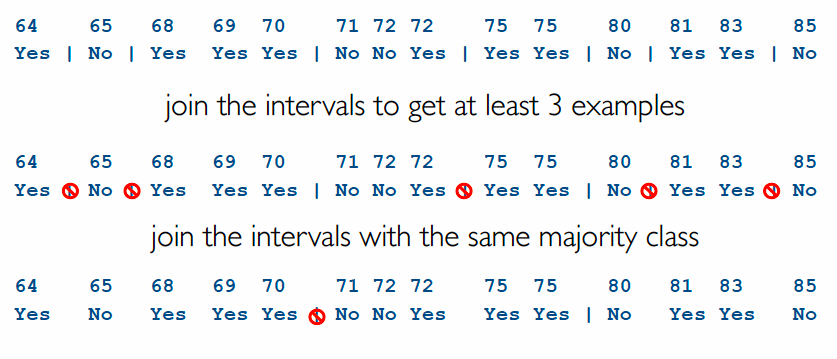
\includegraphics[width=.6\linewidth]{overfittingrules}
\end{figure}

\subsubsection{Sequential Covering}
\begin{enumerate}
\item Take all data and generate one rule
\item \textbf{Eliminate} all \textbf{positive} examples \textbf{covered} by the rule
\item repeat till all examples are covered
\end{enumerate}
\begin{figure}[H]
  \centering
  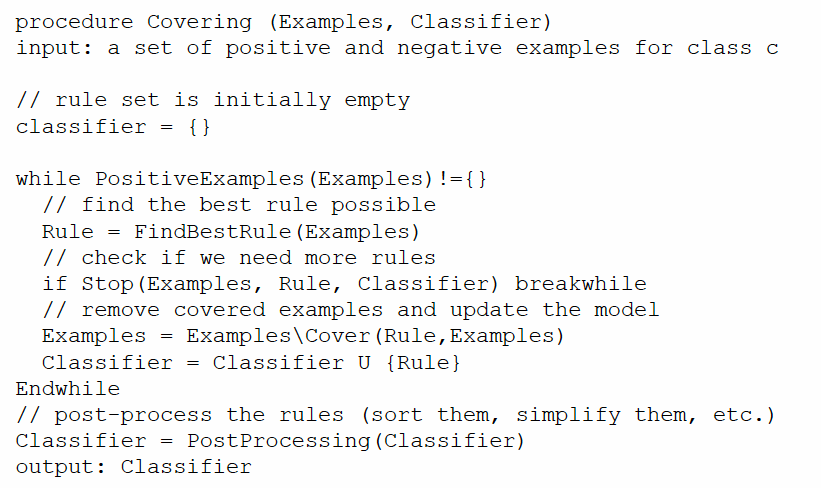
\includegraphics[width=.6\linewidth]{seqcov1}
\end{figure}
\begin{figure}[H]
  \centering
  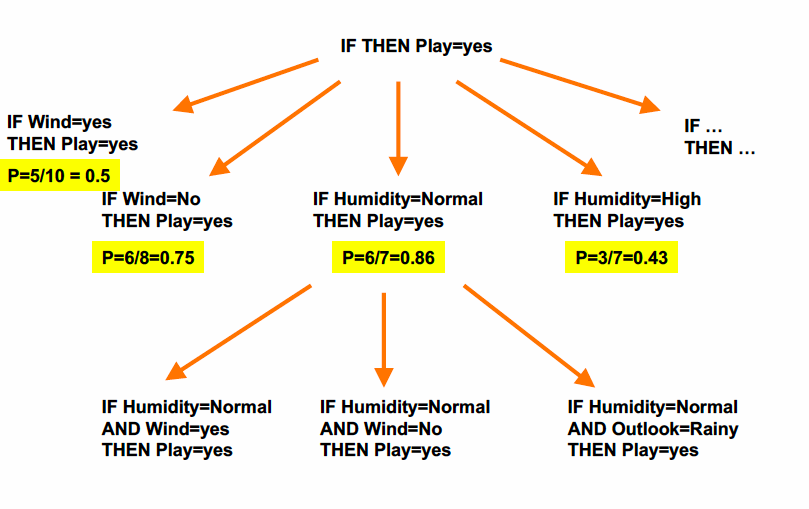
\includegraphics[width=.6\linewidth]{seqcov2}
\end{figure}
This principle is used for example in \textbf{PRISM} :
\begin{figure}[H]
  \centering
  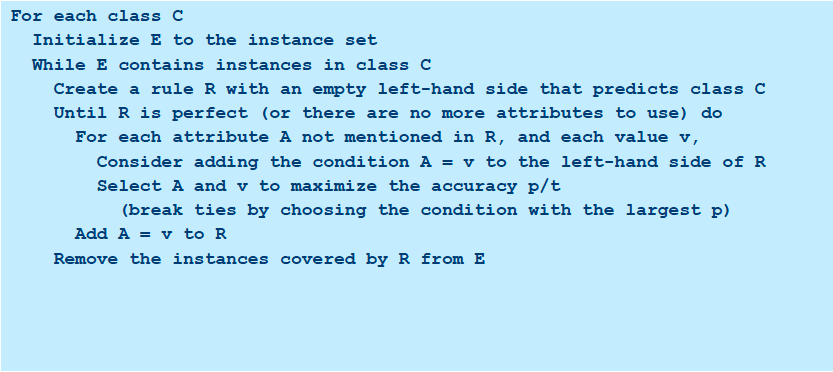
\includegraphics[width=.6\linewidth]{prism}
\end{figure}
Different \textbf{rule testing mechanisms} can be used:
\begin{itemize}
\item \textbf{Accuracy} $\rightarrow \frac{p}{t}$ total over positive, produces rules that cover only positive instances as quick as possible but may produce rule with \textbf{small coverage} (noise?)
\item \textbf{Information gain} $\rightarrow p(log \frac{p}{t}- log \frac{P}{T})$
where P , T are positive and total \textbf{before} the rule was added. 
\end{itemize}
Eliminating covered instances is \textbf{a must} to avoid generating identical rules:
\begin{itemize}
\item Eliminating \textbf{positive} instances ensures that rules are different and that the accuracy is not \textbf{overestimated} which results in a \textbf{robuster} accuracy
\item Eliminating \textbf{negative} instances prevents \textbf{underestimating} the rule's accuracy 
\end{itemize}
\begin{figure}[H]
  \centering
  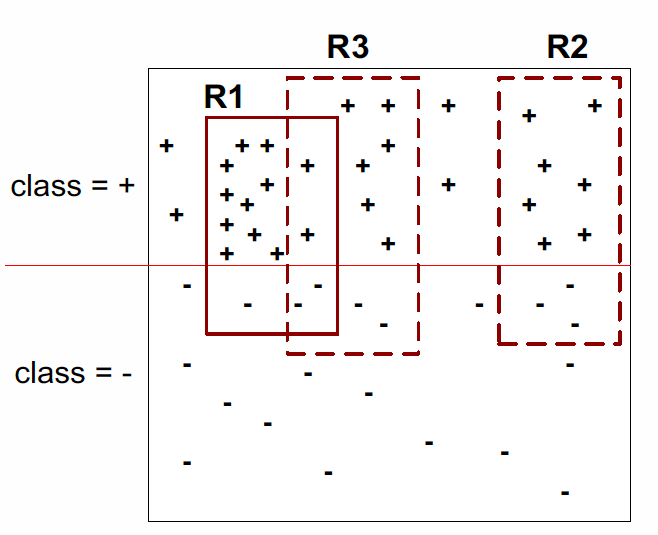
\includegraphics[width=.6\linewidth]{eliminationrules}
\end{figure}
In this case Rule 3 has :
\begin{itemize}
\item \textbf{true score} $\frac{8}{12} = .66$
\item eliminating positive $\frac{6}{10} = .6 < .66 \rightarrow$ \textbf{prevent overestimating}
\item eliminating negative $\frac{8}{10} = .8 > .66 \rightarrow$ \textbf{prevent underestimating}
\end{itemize}

\begin{description}
\item \textbf{Missing values and numeric attributes}\\
Missing values usually \textbf{fail the test} and must be handled in a special way ( for example considering missing as a \textbf{special value}). Otherwise the covering algorithm can \begin{itemize}
\item leave them uncovered until later
\item use other test to test positive examples
\end{itemize}
Numeric attributes are treated just like in DT , with \textbf{binary split points} which can be found by optimizing test selection criterion

\item \textbf{Stopping Criterion and Rule Pruning}\\
The process usually stops when there is \textbf{no} significant improvement by adding a rule ( similar to post-pruning in DT).\\
Reduced error pruning :
\begin{enumerate}
\item Remove \textbf{one conjunct} from a rule
\item Compare error rate on validation set
\item If error improves ,\textbf{prune conjunct}
\end{enumerate}
Pruning can be done using \textbf{incremental pruning} or \textbf{global pruning} using a \textbf{error on holdout set} ,\textbf{statistical significance} or \textbf{MDL principle}.\\
For statistical validity evaluation must be done on data not used for \textbf{growing} the tree : requires \textbf{growing set} and \textbf{pruning set} (split from training set). With the \textbf{reduced error pruning} the algorithm build the full tree on the growing set then prunes it. \textbf{Incremental reduced error pruning} simplifies \textbf{each} rule as soon as it is generated. 
\end{description}

\subsection{Indirect methods}
Rules sets can be far more readable than decision trees (if DT are very complex) . Decision trees also suffer from \textbf{replicated subtrees} .\\Rule sets are collection of \textbf{local models} while trees represents model over the \textbf{whole domain}. The covering algorithm focuses on \textbf{one class at a time} while DT focus on all classes together.